\documentclass[a4paper, 12pt]{article}
\usepackage[a4paper, rmargin=3cm, lmargin=3cm, top=2.5cm, bottom=2.5cm]{geometry}
\usepackage{mathtools}
\usepackage{bookmark}
\usepackage{subcaption}
\usepackage{amsthm,amsmath,amssymb}
\usepackage{enumitem}
\usepackage[ruled, noline]{algorithm2e}
\usepackage{fontspec}

\usepackage{listings} % Para formatar o código
\usepackage{tabularx} % Para tabelas ajustáveis à largura total

\lstset{
    basicstyle=\ttfamily,       % Usa uma fonte monoespaçada
    frame=single,               % Adiciona uma borda ao redor do código
    breaklines=true,            % Quebra linhas automaticamente
    showstringspaces=false      % Não mostra espaços nos strings
}

\usepackage{setspace}
\setstretch{1.5}
\setlength{\parindent}{1.25cm}
\setlength{\parskip}{6px}

\usepackage{unicode-math}
\setmathfont{Stix Two Math}
\setmathfont{TeX Gyre Pagella Math}[
   range=bb,
   Scale=MatchUppercase,
   version=pagella
]

\usepackage{polyglossia}
\setdefaultlanguage{portuguese} % might be portuguese, though referencing may present incompatibilities
\setotherlanguages{english} % secondary language for abstract and stuff
\usepackage{libertine}

% in case you have a local installation for the font Times, this is preferrable, especially if you have Small Caps support
%\setmainfont{times}[
%  % In my case, needs to point for MS Office location since regular MacOS Times doesn't support small caps
%  Path           = /Applications/Microsoft Word.app/Contents/Resources/DFonts/,
%  Extension      = .ttf ,
%  BoldFont       = *bd ,
%  ItalicFont     = *i ,
%  BoldItalicFont = *bi,
%  Ligatures      = Rare, %for some unknown reason, Times put Common ligatures under Rare
%]

% or simply, in case you have the legal font Times LT Std installed in your local machine
%\setmainfont{Times LT Std}[Ligatures = Common] % name might differ

% useful command defition for writting mathematics: QED, norm, set cardinality and equals by definition
\renewcommand{\qedsymbol}{$\blacksquare$}
\newcommand{\norm}[1]{\left\lVert#1\right\rVert}
\newcommand{\card}[1]{\lvert#1\rvert}
\newcommand*{\defeq}{\mathrel{\vcenter{\baselineskip0.5ex \lineskiplimit0pt
                     \hbox{\scriptsize.}\hbox{\scriptsize.}}}%
                     =}

% useful command definition for SCB bracket citation
\newcommand{\citeb}[1]{\bibleftbracket\cite{#1}\bibrightbracket}

% math numbering scheme, speak with your supervisor in case you want to change it
\newtheorem{theorem}{Theorem}[section]
\newtheorem*{definition}{Definition}
\newtheorem{corollary}{Corollary}[theorem]
\newtheorem{lemma}[theorem]{Lemma}


% reference style (Sociedade Brasileira de Computação is compliant with Chicago author-date)
% as per https://presencial.unifcv.edu.br/arquivos/orientacao_para_artigos_area_informatica.pdf
\usepackage[authordate, strict, backend=biber, autolang=other]{biblatex-chicago}
\addbibresource{references.bib}
\DeclareDelimFormat{nameyeardelim}{\addcomma\space}
\setlength\bibitemsep{6.0pt}

% flush all sections right
\usepackage{sectsty}
\sectionfont{\raggedleft}

% used only for text samples, can be safely removed in the final document
\usepackage{lipsum} 
\usepackage{metalogo}

% used for image rendering
\usepackage{graphicx}
\graphicspath{ {../images/} }

\begin{document}
% Page numbering for early pages and document presentation
\pagenumbering{roman}
\setcounter{page}{1}

\thispagestyle{empty}

    \begin{center}
        
\includegraphics[scale=0.18]{../images/unirio.png}\\
        \fontsize{13}{15}
        \textsc{
            Universidade Federal do Estado do Rio de Janeiro\\
            Centro de Ciências Exatas e Tecnológicas\\
            Escola de Informática Aplicada\\
        }
        \vspace{2.8cm}
        Retrieval Augmented Generation Aplicada à Bibliotecas\\
        \vspace{2.8cm}
        Breno Costa da Silva Filgueiras
        \vspace{2.8cm}

        \begin{flushright}
            \textbf{Orientador}\\
            Pedro Nuno de Souza Moura
        \end{flushright}

        \vspace*{\fill}
        
        \textsc{Rio de Janeiro, RJ -- Brasil\\ Dezembro, 2024}
    \end{center}

    \clearpage

    \begin{center}
        Retrieval Augmented Generation Aplicada à Bibliotecas
        \vskip 0.5cm
        Breno Costa da Silva Filgueiras
        \vskip 2.0cm
    \end{center}

    \begin{flushright}
        \parbox{8.0cm}{
        Projeto de graduação apresentado à Escola de Informática Aplicada
        da Universidade Federal do Estado do Rio de Janeiro (UNIRIO) como
        cumprimento de requerimento parcial para obtenção título de Bacharel em
        Sistemas de Informação.}
        \vskip 1.5cm
        Approved by:
        \vskip 1.5cm
        \rule{10.0cm}{.1mm}

        Pedro Nuno de Souza Moura -- UNIRIO
        \vskip 1.0cm
        
        \rule{10.0cm}{.1mm}

        Supervisor 2, D.Sc. -- UNIRIO
        \vskip 1.0cm

        \rule{10.0cm}{.1mm}

        Supervisor 3, D.Sc. -- XXXX
        \vskip 1.0cm
    \end{flushright}
    \vspace{\stretch{1}}
    \begin{center}
        \textsc{Rio de Janeiro, RJ -- Brasil} \\ \textsc{Dezembro, 2024}
    \end{center}
    % Fim da folha de rosto

    \clearpage
    \begin{flushright}
        Agradecimentos
    \end{flushright}
    \lipsum[1-2]

    \clearpage

    \begin{abstract}
        Em uma parceria entre Seagate e a International Data Corporation (IDC) foi realizado o estudo \citetitle{digitization}, nele a IDC fala sobre diversos aspectos referentes aos dados presentes no mundo digital e um dos tópicos abordados no estudo é “Mankind is on a quest to digitize the world” e neste mesmo tópico eles explicam que os dados que geramos no dia a dia está em constante crescimento, ou seja, estamos gradualmente produzindo mais dados.

        Com um volume cada vez maior de dados, uma busca por informação otimizada é essencial, dado que são necessárias ferramentas que nos garantam confiança e precisão da informação adquirida. Com isso em mente, este trabalho visa o desenvolvimento de um sistema capaz de ler, processar e armazenar documentos diversos de determinada biblioteca (conjunto de documentos) para que possamos utilizar um \textit{Large Language Model} (LLM) para responder perguntas que os usuários possam ter acerca dos documentos.
        
        A ideia é conseguir processar documentos de diferentes épocas, temas, formatos e conseguir responder o maior número possível de perguntas dos usuários com a melhor confiança possível.

        \begin{flushleft}
            \textbf{Palavras-chave:} retrieval, augmented, generation, inteligência, artificial.
        \end{flushleft}
    \end{abstract}
    \clearpage

    \begin{english}
        \begin{abstract}
            In a partnership between Seagate and the International Data Corporation (IDC), the study \citetitle{digitization} was conducted. In it, IDC discusses various aspects related to data present in the digital world and one of the topics covered in the study is “Mankind is on a quest to digitize the world”. In this same topic, they explain that the data we generate on a daily basis is constantly growing, that is, we are gradually producing more data.

            With an ever-increasing volume of data, an optimized search for information is essential, given that tools are needed that guarantee reliability and accuracy of the information acquired. With this in mind, this work aims to develop a system capable of reading, processing and storing various documents from a given library (set of documents) so that we can use a \textit{Large Language Model} (LLM) to answer questions that users may have about the documents.

            The idea is to be able to process documents from different periods, themes and formats and to be able to answer as many user questions as possible with the greatest possible confidence.

            \begin{flushleft}
                \textbf{Keywords:} retrieval, augmented, generation, artifical, inteligence.
            \end{flushleft}
        \end{abstract}
    \end{english}
    \clearpage

    \tableofcontents
    \clearpage

    \listoffigures
    \clearpage

    \listoftables
    \clearpage

    % \listofalgorithms
    % \clearpage

    \pagenumbering{arabic}
    \setcounter{page}{1}

    \section{Introdução}

    Com a expansão contínua da Internet das Coisas (IoT), o cenário se transforma em um redemoinho de informações. Chegará, ou talvez já tenha chegado, o momento em que será impossível para qualquer ser humano consumir tudo o que criou em um único dia.

    Durante estudo, a \textit{International Data Coorporation} (IDC) previu que a \textit{Global Datasphere} cresceria de 45 zettabytes em 2019 para 175 zettabytes em 2025 \citeb{digitization}. Um crescimento de aproximadamente 380\% em 6 anos, porém essa previsão foi feita em 2018 e atualmente já existem estudos que projetam números ainda maiores para a produção de dados. Como é o exemplo do estudo \citetitle{data_created}, onde foram calculados um total de 147 \textit{zetabytes} produzidos em 2024, com previsão de 181 \textit{zetabytes} para 2025, um crescimento de 23.12\% \citeb{data_created}.

    \begin{figure}[h]
        \label{fig:total_dados_anual}
        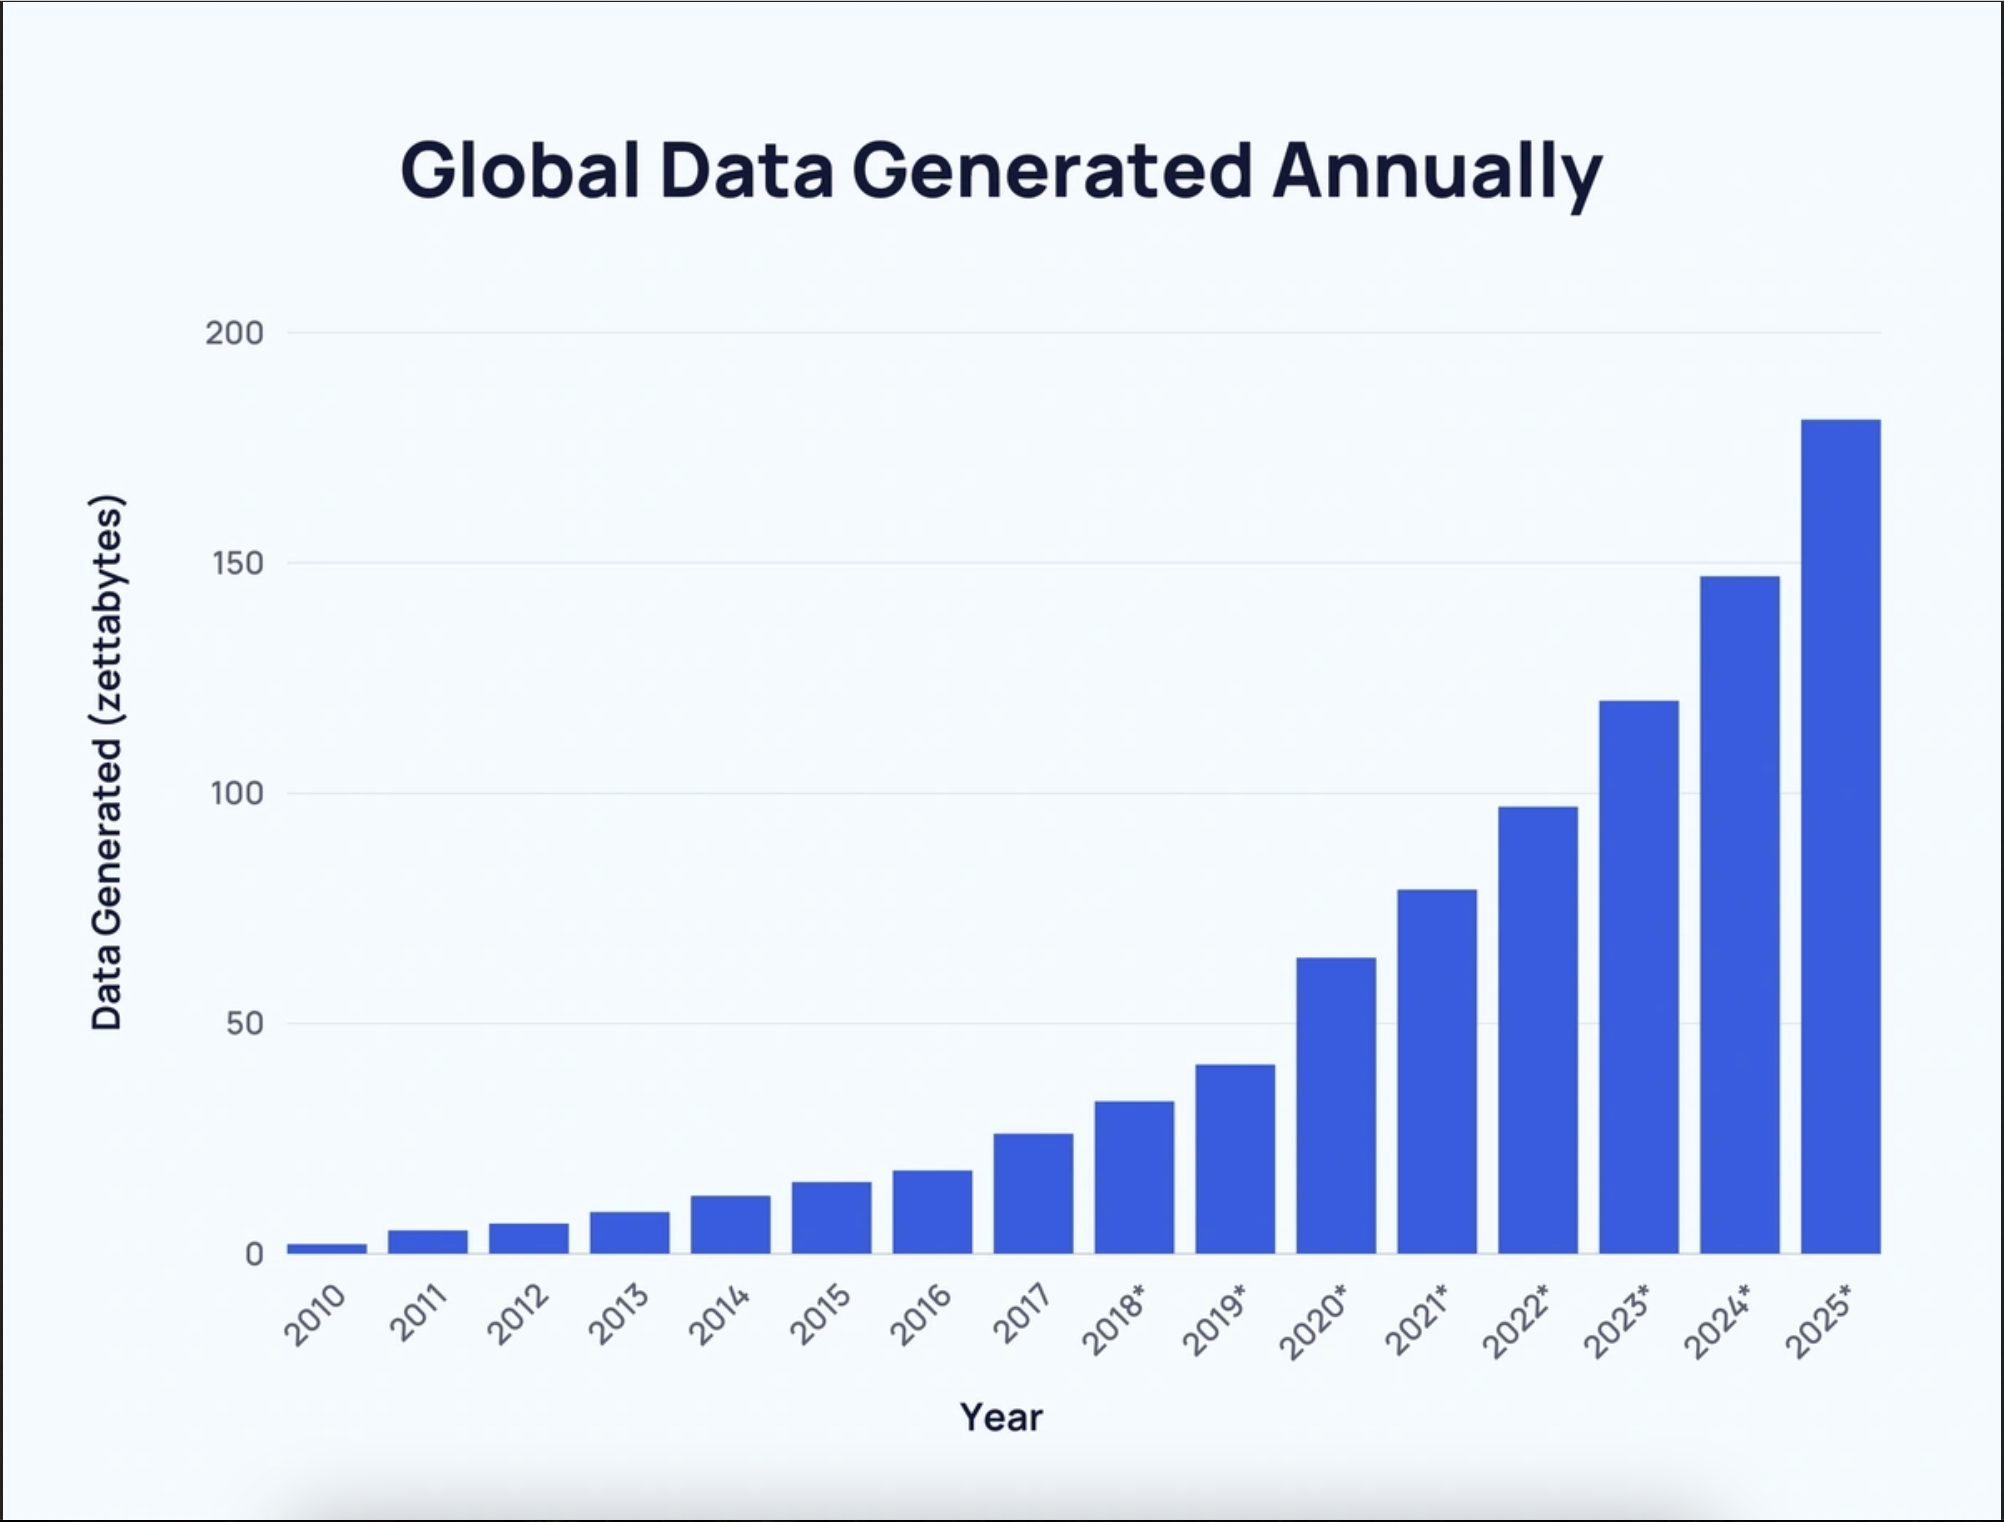
\includegraphics[width=\textwidth,height=0.9\textheight,keepaspectratio]{global-data-generated-annually-fabio-duarte.png}
        \centering
        \caption{Total de dados produzidos por ano, \citeb{data_created}}
        \centering
    \end{figure}        

    \subsection{Motivação}

    No estudo \citetitle{digitization}, a \textit{Seagate}, gigante do armazenamento de dados, uniu forças com a \textit{International Data Corporation} (IDC) para conduzir uma análise dos dados presentes na \textit{Global Datasphere}, que quantifica e analisa o total de dados criados, capturados e replicados no mundo inteiro. A IDC destacou: \textit{“Mankind is on a quest to digitize the world.”} Essa frase encapsula a era em que vivemos, marcada por um crescimento incessante no volume de dados que produzimos diariamente.
    
    Cada clique, pagamento por aproximação ou uso de \textit{wearables} adiciona mais um fragmento ao vasto oceano digital. Nesse turbilhão de dados, buscar uma matéria ou reportagem torna-se uma tarefa semelhante a encontrar uma agulha em um palheiro digital, um desafio tão fascinante quanto frustrante.

    E esse contexto de imensidão de dados onde a busca por informações é cada vez mais dificíl, é o berço deste projeto. O objetivo é implementar uma solução que processe bibliotecas de documentos e aplique o conceito de \textit{Retrieval Augmented Generation} (RAG). Com uma interface de chat simples, o usuário poderá fazer perguntas e receber respostas humanizadas, geradas por um \textit{Large Language Model} (LLM), com referências claras aos documentos de origem.

    O desafio de buscar informações relevantes é significativo. A internet ainda abriga dados sem referência ou apresentados de formas variadas, como gráficos e textos, dificultando a assimilação. Além disso, interfaces pouco intuitivas e mecanismos de busca ineficazes consomem tempo valioso. Para estudantes e pesquisadores, essa batalha constante com a desorganização digital pode transformar o simples ato de encontrar informações em um verdadeiro labirinto.

    \subsection{Objetivos}

    O objetivo principal deste trabalho é implementar uma solução baseada em \textit{Retrieval Augmented Generation} (RAG) para bibliotecas de documentos específicos, a fim de viabilizar consultas que retornem dados pertinentes junto com suas referências. Os objetivos específicos são:
    
    \begin{enumerate}
        \item Escrever uma introdução acessível ao conceito de RAG aos alunos do BSI.
        \item Produzir um documento que instrua a implementação de um ecossistema RAG aos alunos do BSI.
        \item Realizar a implementação de RAG para documentos, que seja agnóstica tanto ao LLM quanto embeeding utilizados.
        \item Executar uma validação sobre a solução gerada, de maneira que o resultado seja relevante.
    \end{enumerate}

    \subsection{Organização do Texto}

    Este trabalho está organizado em capítulos, com o objetivo de apresentar os processos, métodos, análises e descobertas de forma clara e coerente. A estrutura do documento foi elaborada para facilitar a compreensão do leitor sobre a complexidade do tema e os resultados obtidos, conduzindo-o até a implementação da solução final. Os capítulos estão estruturados da seguinte forma:
    
    \begin{itemize}
        \item \textbf{Introdução:} Apresenta o contexto do trabalho, destacando o problema do crescente volume de dados. Discute a motivação para a solução proposta, sua relevância no cenário atual e os objetivos estabelecidos.
        \item \textbf{Conceitos Fundamentais:} Dedica-se à fundamentação teórica, abordando os conceitos essenciais para a compreensão da solução e sua implementação. Inclui uma introdução ao conceito de \textit{Large Language Models} (LLM) e uma análise detalhada do \textit{Retrieval Augmented Generation} (RAG).
        \item \textbf{Modelagem:} Descreve a composição da solução, explicando os artefatos envolvidos e suas responsabilidades. Também aborda o funcionamento e o papel de cada componente na solução final. Ao final, apresenta as tecnologias utilizadas, incluindo descrições breves sobre as ferramentas, suas versões e funções.
        \item \textbf{Solução Desenvolvida:} Detalha os artefatos implementados, explicando como a solução cumpre suas funções. Apresenta os resultados obtidos e discute as respostas fornecidas para algumas das questões propostas, avaliando a eficácia da solução.
        \item \textbf{Conclusão:} O capítulo final resume as considerações sobre os resultados alcançados, destacando tanto os aspectos positivos quanto as limitações da solução implementada. Além disso, discute possíveis trabalhos futuros ou aplicações derivadas da solução, encerrando com as referências utilizadas no desenvolvimento do trabalho.
    \end{itemize}

    \subsection{Metodologia}

    Este trabalho adotará a abordagem de \textit{Design Science Research} (DSR) para garantir que ao final do trabalho, o artefato modelado esteja implementado e funcionando conforme planejado.

    O DSR, possui raízes na engenharia e nas ciências do artificial \citeb{simon_1996}, é uma metodologia voltada para a resolução de problemas. Seu objetivo é aprimorar o conhecimento humano por meio da criação de artefatos inovadores e da geração de conhecimento de design, oferecendo soluções práticas para problemas do mundo real \citeb{design_science}.

    Assim, ao utilizar o \textit{Design Science Research} (DSR), este trabalho resultará em um artefato produzido com base nas análises e discussões realizadas ao longo das próximas seções deste trabalho.
    
    \clearpage

    \section{Conceitos Fundamentais}

    Para que este trabalho seja compreendido e os próximos capítulos possam ser apresentados com maior clareza, é necessário passarmos por alguns conceitos. Antes de nos aprofundarmos no contexto de um ecossistema de \textit{retrieval augmented generation} (RAG), é necessário compreender um pouco a IA generativa e os \textit{Large Language Models} (LLMs) que contribuem tanto para a interpretação das perguntas feitas durante as interações com o usuário, quanto na geração de uma resposta mais humana.
    
    \subsection{IA Generativa}
    
    A inteligência artificial generativa, às vezes chamada de \textit{gen AI}, é um tipo de inteligência artificial (IA) capaz de criar conteúdo original — como texto, imagens, vídeos, áudio ou código de software — em resposta a um comando ou solicitação do usuário. \citeb{genai_ibm}

    A inteligência artificial generativa baseia-se em modelos avançados de \textit{machine learning} (aprendizado de máquina) chamados modelos de \textit{deep learning} (aprendizagem profunda) — algoritmos que simulam os processos de aprendizado e tomada de decisão do cérebro humano. Esses modelos trabalham identificando e codificando padrões e relações em grandes volumes de dados.

    A partir dessas informações, a IA generativa é capaz de compreender solicitações ou perguntas feitas em linguagem natural pelos usuários, respondendo com conteúdos novos e relevantes. Essa capacidade permite a criação de textos, imagens, vídeos, áudios e até códigos de software, de forma original e adaptada ao pedido do usuário.

    \subsubsection{Uma Breve História da IA Generativa}

    O termo "IA generativa" explodiu na consciência pública na década de 2020, mas a IA generativa já faz parte de nossas vidas há décadas, e a tecnologia de IA generativa atual se baseia em avanços de aprendizado de máquina que remontam ao início do século 20. Uma história representativa não exaustiva da IA generativa pode incluir algumas das seguintes datas:

    \begin{itemize}
        \item \textbf{1964:} O cientista da computação do \textit{Massachusetts Institute of Technology} (MIT), Joseph Weizenbaum, desenvolve o ELIZA, uma aplicação de processamento de linguagem natural baseada em texto. Essencialmente o primeiro \textit{chatbot} (chamado de \textit{"chatterbot"} na época), o ELIZA usava \textit{scripts} de correspondência de padrões para responder a entradas de linguagem natural digitadas com respostas empáticas em texto.

        \item \textbf{1999:} A Nvidia lança o GeoForce, a primeira unidade de processamento gráfico (GPU). Originalmente desenvolvida para fornecer gráficos de movimento suave para videogames, as GPUs se tornaram a plataforma padrão para o desenvolvimento de modelos de IA e mineração de criptomoedas.

        \item \textbf{2004:} O Google \textit{autocomplete} aparece pela primeira vez, gerando palavras ou frases potenciais à medida que os usuários digitam seus termos de busca.

        \item \textbf{2013:} Aparecem os primeiros \textit{autoencoders} variacionais (VAEs).

        \item \textbf{2014:} Surgem as primeiras redes adversariais generativas (GANs) e modelos de difusão.

        \item \textbf{2017:} Ashish Vaswani, uma equipe do Google Brain e um grupo da Universidade de Toronto publicam o artigo \textit{Attention is All you Need}, \citeb{att_all_u_need}, um artigo que documenta os princípios dos modelos de transformadores, amplamente reconhecidos como os responsáveis por permitir os modelos de fundação mais poderosos e as ferramentas de IA generativa que estão sendo desenvolvidas hoje.

        \item \textbf{2019-2020:} O OpenAI lança seus modelos de linguagem GPT (\textit{Generative Pre-trained Transformer}), o GPT-2 e o GPT-3.

        \item \textbf{2022:} O OpenAI apresenta o ChatGPT, uma interface do GPT-3 que gera frases complexas, coerentes e contextuais, além de conteúdo de longo formato em resposta a comandos dos usuários.
        
        \item \textbf{2023-2024:} Com a notoriedade e popularidade do ChatGPT, que efetivamente abriu as portas para uma onda de desenvolvimentos, os avanços e lançamentos de produtos em IA generativa têm ocorrido a um ritmo acelerado, incluindo lançamentos do Google Bard (agora Gemini), Microsoft Copilot, IBM watsonx.ai e o modelo de linguagem Llama-2 de código aberto da Meta.
    \end{itemize}

    \subsubsection{Mais à Frente}

    A inteligência artificial tem sido um tema relevante na tecnologia, mas foi a IA generativa, especialmente com o lançamento do ChatGPT em 2022, que a destacou globalmente, gerando inovação e adoção. Ela oferece grandes benefícios de produtividade para indivíduos e organizações, e, apesar dos desafios e riscos, as empresas exploram como melhorar fluxos de trabalho e enriquecer produtos e serviços. De acordo com uma pesquisa da consultoria \textit{McKinsey}, mais de 65\% das empresas usam Gen AI no mundo. \citeb{mckinsey_genai}.

    \subsection{Large Language Models}

    Os \textit{Large Language Models} (LLMs) são uma categoria de modelos fundamentais treinados em grandes volumes de dados para oferecer capacidades versáteis, atendendo a diversos casos de uso e tarefas. Diferentemente dos modelos específicos para determinados domínios, que exigem treinamentos separados para cada aplicação—geralmente com altos custos e demandas significativas de infraestrutura—os LLMs promovem uma aplicação mais ampla, gerando sinergias entre diferentes áreas e, muitas vezes, alcançando um desempenho superior. \citeb{llm_ibm}

    Os LLMs representam um avanço significativo em \textit{Natural Language Processing} (NLP) e inteligência artificial. Esses modelos estão amplamente acessíveis ao público por meio de interfaces como o \textit{ChatGPT-3} e \textit{GPT-4} da \textit{OpenAI}, apoiados pela \textit{Microsoft}. Outros exemplos incluem os modelos \textit{Llama} da Meta, os modelos \textit{BERT/RoBERTa} e \textit{PaLM} do Google, e a série \textit{Granite} lançada pela IBM.

    Os LLMs são projetados para compreender e gerar texto de forma similar à humana, além de produzir outros tipos de conteúdo. Com base nos extensos volumes de dados em que foram treinados, conseguem traduzir idiomas, resumir textos, responder perguntas, auxiliar na redação e até mesmo na geração de código.

    Essas capacidades são viabilizadas por bilhões de parâmetros que capturam padrões complexos da linguagem. Como resultado, os LLMs estão transformando áreas como chatbots, assistentes virtuais, geração de conteúdo, suporte à pesquisa e tradução de idiomas.

    \subsubsection{Como funcionam?}

    Os \textit{Large Language Models} (LLMs) operam utilizando técnicas de aprendizagem profunda e grandes volumes de dados textuais. Baseados na arquitetura de transformadores \citeb{att_all_u_need}, como o \textit{Generative Pre-trained Transformer} (GPT), esses modelos são especialmente eficazes em lidar com dados sequenciais, como entradas de texto. Compostos por várias camadas de redes neurais, os LLMs empregam um mecanismo de atenção para focar em partes específicas dos conjuntos de dados.

    Durante o treinamento, os modelos aprendem a prever a próxima palavra em uma sentença com base no contexto fornecido pelas palavras anteriores. Isso é feito atribuindo probabilidades à recorrência de palavras que foram tokenizadas (divididas em sequências menores) e transformadas em embeddings, representações numéricas do contexto.

    O treinamento envolve o uso de corpora massivas, com bilhões de páginas de texto, permitindo que os LLMs aprendam gramática, semântica e relações conceituais por meio de aprendizado auto-supervisionado e técnicas de zero-shot. Uma vez treinados, os modelos geram texto prevendo autonomamente a próxima palavra com base na entrada recebida e nos padrões adquiridos, resultando em uma produção linguística coerente e relevante para diversas tarefas de compreensão e geração de linguagem.

    O desempenho dos LLMs pode ser aprimorado por meio de técnicas como \textit{prompt engineering}, \textit{fine-tuning} (ajuste fino) e aprendizado por reforço com feedback humano (\textit{RLHF}). Essas abordagens ajudam a mitigar problemas como vieses, discurso de ódio e respostas incorretas ou ilusórias (\textit{hallucinations}), que podem surgir devido ao treinamento em dados não estruturados. Garantir que os LLMs estejam prontos para uso em nível corporativo é crucial para evitar riscos à reputação e responsabilidades indesejadas.


    \subsection{O Problema}

    No livro \citetitle{rothman}, é dito que ``mesmo o modelo mais avançado de Inteligência Artificial (IA) generativa é limitado a responder somente sobre dados nos quais ele foi treinado.'' \citeb{rothman}. Essa afirmação chama a atenção para um problema especial: como fazer para que uma IA saiba responder perguntas referentes a um conjunto específico de dados, diferente daquele em que foi treinada?

    Quando um modelo de IA generativo não sabe como responder com precisão, alguns dizem que ele está produzindo viés ou sofrendo uma \textit{hallucination} (alucinação). No entanto, ``tudo se resume à impossibilidade de fornecer uma resposta adequada quando o treinamento do modelo não incluiu as informações solicitadas além dos problemas clássicos de configuração do modelo.'' \citeb{rothman}. Essa confusão geralmente leva a sequências aleatórias das saídas mais prováveis, não das mais precisas.

    Buscando mitigar essas questões, em 2020 foi publicado o artigo \citetitle{RAG} \citeb{RAG}, que combinava abordagens baseadas em recuperação com modelos generativos, introduzindo a \textit{Retrieval Augmented Generation} (RAG). Uma RAG recupera dados relevantes de fontes externas em tempo real e usa esses dados para gerar respostas contextualmente relevantes, isto é, que façam sentido dentro do contexto trabalhado durante as consultas feitas pelo usuário. Uma de suas principais vantagens é a adaptabilidade, tendo em vista que a estrutura pode ser aplicada independente do tipo de dado abordado na solução, seja texto, imagens, áudios ou documentos diversos.


    \subsection{Retrieval Augmented Generation (RAG)}
    
    Quando um modelo de IA generativa não sabe responder determinada pergunta com precisão, diz-se que ele está alucinando ou apresentando viés, mas, na prática, está apenas gerando respostas sem sentido. Isso ocorre porque o modelo não foi treinado com as informações solicitadas ou por conta de limitações em sua configuração, resultando em sequências prováveis, mas não precisas necessariamente.

    Uma RAG começa onde a IA generativa termina, fornecendo informações que um modelo de LLM não possui para responder com precisão as consultas do usuário. Uma RAG otimiza tarefas de recuperação de informações e adiciona os dados recuperados durante a entrada (seja consulta do usuário ou um prompt automatizado), gerando uma saída melhorada e mais amigável ao usuário. O funcionamento geral da RAG pode ser resumido na \ref{fig:rag_estudante}, que será explicada nos próximos parágrafos:

    \begin{figure}[h]
        \label{fig:rag_estudante}
        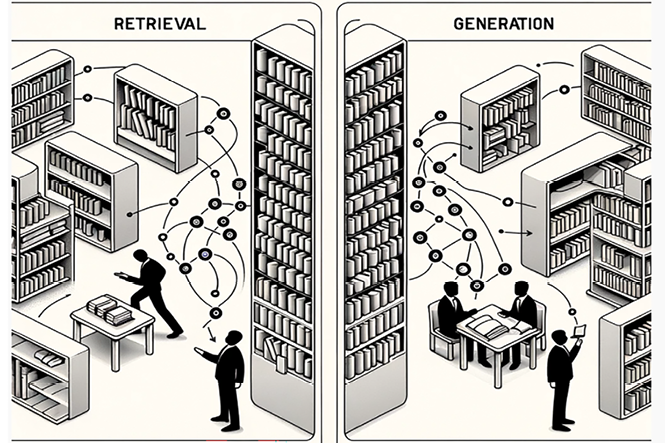
\includegraphics[width=\textwidth,height=0.9\textheight,keepaspectratio]{retrieval-generation-denis-rothman.png}
        \centering
        \caption{Funcionamento geral de uma estrutura RAG (extraída de \citeb{rothman})}
        \centering
    \end{figure}

    Imagine um estudante em uma biblioteca, com a tarefa de escrever uma dissertação sobre RAG. Assim como o ChatGPT ou outras ferramentas de IA generativa, o estudante sabe ler e escrever. Como qualquer LLM, o estudante é treinado para compreender informações avançadas, resumir e criar conteúdo. No entanto, como qualquer IA, há muitas informações que este estudante ainda desconhece.

    Na fase de recuperação, ele busca por livros sobre o tema necessário (lado esquerdo da \ref{fig:rag_estudante}) na biblioteca. Em seguida, ele retorna ao seu lugar, realiza a tarefa de recuperação sozinho ou com a ajuda de um colega, extraindo as informações relevantes dos livros adquiridos. Na fase de geração (lado direito da \ref{fig:rag_estudante}), o estudante começa a escrever a sua dissertação utilizando o conhecimento adquirido na fase anterior. Esse é o funcionamento de um agente humano guiado por RAG, de maneira semelhante a uma estrutura de IA generativa baseada em RAG.

    Enquanto escreve sua dissertação sobre RAG, o estudante encontra tópicos difíceis com os quais não tem tempo para consultar todas as informações disponíveis. Como um agente humano generativo, ele fica travado, assim como um modelo de IA generativa. Ele até pode tentar escrever algo sobre esses tópicos, mas, como a IA, não saberá se o conteúdo está correto até que alguém corrija a dissertação e lhe avalie de alguma maneira.

    Neste ponto, ele já atingiu seu limite e decide recorrer a uma ferramenta de IA generativa com RAG para obter respostas corretas e auxiliá-lo. No entanto, existe uma grande variedade de modelos de LLM e configurações RAG disponíveis, deixando o estudante sobrecarregado. Antes de prosseguir, é necessário entender os recursos disponíveis e como o RAG está organizado.

    \subsection{Ecossistema RAG}

    A IA generativa baseada em RAG é um \textit{framework} que pode ser implementada com diversas configurações, funcionando dentro de um ecossistema amplo (\ref{fig:arquitetura_rag}). Independentemente da quantidade de estruturas de recuperação e geração disponíveis, tudo se resume a quatro eixos principais e suas respectivas questões:
    
    \begin{itemize}
        \item \textbf{Dados:} De onde vêm os dados? São confiáveis e suficientes? Há questões de direitos autorais, privacidade ou segurança?
        \item \textbf{Armazenamento:} Como os dados serão armazenados antes ou depois do processamento? Qual será o volume armazenado?
        \item \textbf{Recuperação:} Como os dados corretos serão recuperados para complementar a entrada (ou consulta) do usuário? Qual tipo de \textit{framework} RAG será mais adequado ao projeto?
        \item \textbf{Geração:} Qual modelo de IA generativa melhor se adapta ao \textit{framework} RAG escolhido?
    \end{itemize} 

    Esses eixos dependem do tipo de \textit{framework} RAG utilizado. Antes de escolher, é essencial avaliar a proporção de conhecimento paramétrico e não paramétrico no ecossistema implementado. No contexto de aprendizado de máquina, o conhecimento paramétrico é o entendimento internalizado que um modelo ganha com o treinamento em um conjunto de dados. 
    
    Esse conhecimento é representado pelos parâmetros do modelo (pesos e vieses), que são ajustados durante o processo de treinamento para minimizar a função de perda e melhorar o desempenho do modelo. O Conhecimento paramétrico permite que o modelo faça previsões e generalize para dados novos e invisíveis, capturando recursos e relacionamentos essenciais dentro dos dados de treinamento.
    
    Nos próximos parágrafos, a \ref{fig:arquitetura_rag} abaixo, ilustrando os principais componentes do \textit{framework} RAG (independentemente do tipo implementado), será explicada.

    \begin{figure}[h]
        \label{fig:arquitetura_rag}
        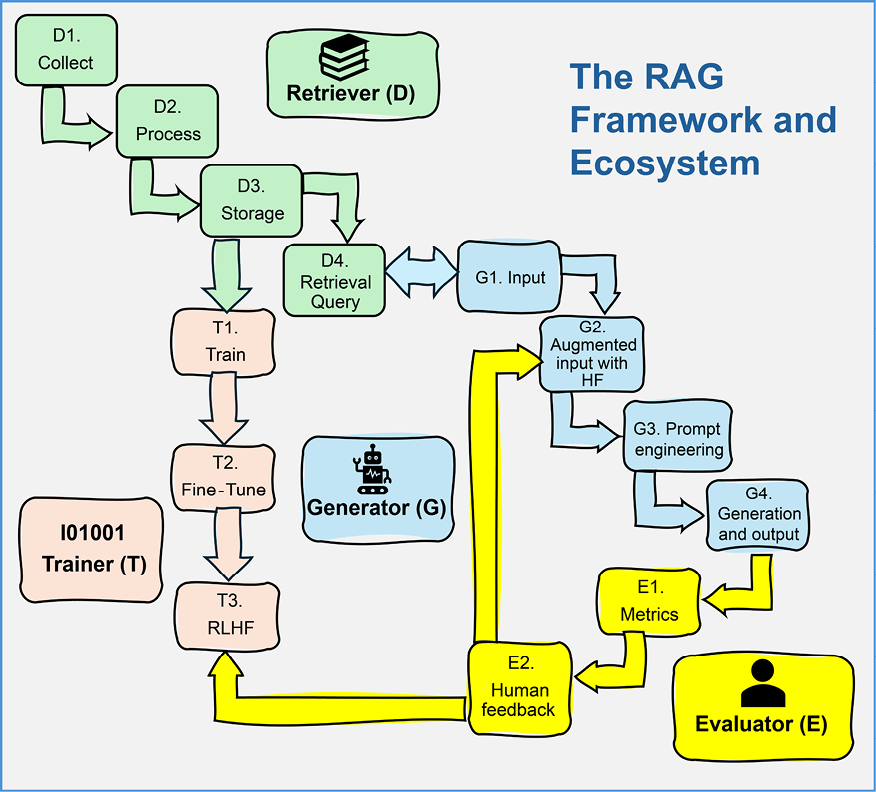
\includegraphics[width=\textwidth,height=0.9\textheight,keepaspectratio]{rag-framework-ecosystem-denis-rothman.png}
        \centering
        \caption{Arquitetura da estrutura RAG (extraída de \citeb{rothman})}
        \centering
    \end{figure}

    \begin{itemize}
        \item \textbf{\textit{Retriever} (D, em verde na \ref{fig:arquitetura_rag}):} Responsável pela coleta, processamento, armazenamento e recuperação de dados.
        \item \textbf{\textit{Generator} (G, em azul na \ref{fig:arquitetura_rag}):} Cuida da complementação da entrada, engenharia de prompts e geração de respostas.
        \item \textbf{\textit{Evaluator} (E, em amarelo na \ref{fig:arquitetura_rag}):} Avalia o desempenho usando métricas matemáticas, \textit{feedback} humano e outras formas de validação.
        \item \textbf{\textit{Trainer} (T, em rosa na \ref{fig:arquitetura_rag}):} Gerencia o modelo pré-treinado inicial e sua posterior ajuste fino (\textit{fine-tuning}).
    \end{itemize}

    Esses quatro componentes dependem de seus respectivos ecossistemas, composto por seus subcomponentes, formando o \textit{pipeline} de IA generativa baseada em RAG. Nas seções a seguir, serão usadas as siglas D, G, E e T para representar,respectivamente, \textit{Retriever}, \textit{Generator}, \textit{Evaluator} e \textit{Trainer}.

    \subsubsection{\textit{Retriever} (D)}

    O componente \textit{retriever} de um ecossistema RAG coleta, processa, armazena e recupera dados. O ponto de partida de um ecossistema RAG é, portanto, um processo de ingestão de dados, cujo primeiro passo é a coleta de dados. Os subcomponentes são:

    \begin{enumerate}
        \item \textbf{Coleta de Dados (D1):} Atualmente dados são extremamente diversos, podendo ser textos, arquivos de mídia (como músicas ou vídeos em mp4) ou arquivos estruturados e não estruturados (PDFs, JSONs e páginas \textit{web}). Além disso, grande parte desses dados é não estruturada e pode ser encontrada de maneiras imprevisíveis e complexas. Felizmente, várias plataformas, como Pinecone\footnote{Disponível em \citeb{pinecone}}, OpenAI\footnote{Disponível em \citeb{openai}}, Chroma\footnote{Disponível em \citeb{chroma}} e Activeloop\footnote{Disponível em \citeb{activeloop}}, oferecem ferramentas prontas para processar e armazenar essa vasta quantidade de dados.
        \item \textbf{Processamento de Dados (D2):} Na fase de coleta de dados (D1) no processamento de dados multimodais, diferentes tipos de dados, como texto, imagens e vídeos, podem ser extraídos de \textit{websites} utilizando técnicas de \textit{web scraping} ou outras fontes de informação. Esses objetos de dados são então transformados para criar representações uniformes. Alguns exemplos dessas transformações incluem: \textit{chunking}, \textit{embedding} e indexação. Essas técnicas serão discutidas mais adiante.
        \item \textbf{Armazenamento de Dados (D3):} Neste estágio do \textit{pipeline}, já se coletou e se iniciou o processamento de uma grande quantidade de dados diversos. Mas para fazermos com que esses dados sejam úteis, deve-se fazer uso de \textit{vector stores} (armazenamento de vetores), como Elastic Search. Esse não apenas armazena os dados, mas os convertem em entidades matemáticas, representadas como vetores, permitindo realizar cálculos poderosos. Esses sistemas também utilizam técnicas de indexação e outras abordagens para garantir acesso rápido e eficiente aos dados. Em vez de manter os dados em arquivos estáticos, transforma-se tudo em um sistema dinâmico e pesquisável, pronto para alimentar \textit{chatbots}, motores de busca e outras aplicações.
        \item \textbf{Consulta de Recuperação (D4):} O processo de recuperação é acionado pela entrada (ou consulta) do usuário ou entrada automatizada (G1). Para recuperar dados rapidamente, carregamos os dados nos \textit{vector stores} e \textit{datasets} após transformá-los para um formato adequado. Em seguida, utilizamos uma combinação de pesquisas por palavras-chave, \textit{embeddings} inteligentes e indexação para recuperar os dados de forma eficiente.
        A similaridade cosseno, que calcula o cosseno entre dois vetores, por exemplo, encontra itens (vetores) que estejam intimamente relacionados, garantindo que os resultados da busca não sejam apenas rápidos, mas também altamente relevantes.
        Após a recuperação dos dados, o próximo passo é aumentar a entrada, ou seja, adicionar as informações recuperadas para enriquecer a resposta gerada ao usuário.
    \end{enumerate}

    \subsubsection{\textit{Generator} (G)}

    No ecossistema RAG, as linhas entre a entrada e a recuperação não são tão nítidas, como mostrado na \ref{fig:arquitetura_rag}, que representa o \textit{framework} e ecossistema RAG. A entrada do usuário (G1), seja automatizado ou humano, interage com a consulta de recuperação (D4) para complementar a entrada antes de enviá-la ao modelo generativo. O fluxo gerativo começa com a entrada do usuário, que é aprimorada com dados recuperados antes de ser processada pelo modelo de IA generativa.

    \begin{enumerate}
        \item \textbf{Entrada (G1):} A entrada pode ser uma série de tarefas automatizadas (como o processamento de \textit{e-mails}, por exemplo) ou \textit{prompts} humanos por meio de uma Interface de Usuário (\textit{User Interface} - UI). Essa flexibilidade permite integrar a IA de forma flúida em diversos ambientes profissionais, aprimorando a produtividade em diferentes setores.
        \item \textbf{Entrada Aumentada com Feedback Humano (G2):} O feedback humano (\textit{Human Feedback} - HF) pode ser adicionado à entrada, conforme descrito na seção \ref{human_feedback}, sob o componente \textit{evaluator} (E). O \textit{feedback} humano torna o ecossistema RAG consideravelmente mais adaptável, permitindo total controle sobre a recuperação de dados e as entradas para a IA generativa.
        \item \textbf{Engenharia de \textit{Prompts} (G3):} Tanto o \textit{retriever} (D) quanto o \textit{generator} (G) dependem fortemente da engenharia de \textit{prompts} para preparar a mensagem padrão e aumentada que o modelo de IA generativa deverá processar. A engenharia de \textit{prompts} combina a saída do \textit{retriever} (D) com a entrada do usuário, garantindo que o modelo receba uma entrada bem estruturada e relevante para gerar a resposta desejada.
        \item \textbf{Geração e Saída (G4):} A escolha de um modelo de IA generativa (LLM) depende dos objetivos do projeto. Modelos como Llama\footnote{Disponível em \citeb{llama_models}}, Gemini\footnote{Disponível em \citeb{gemini_models}}, GPT\footnote{Disponível em \citeb{gpt_models}} e outros podem atender a diferentes requisitos. No entanto, o \textit{prompt} precisa estar alinhado com as especificações de cada modelo.
    \end{enumerate}

    \subsubsection{\textit{Evaluator} (E)}

    Frequentemente, dependemos de métricas matemáticas para avaliar o desempenho de um modelo de IA generativa (LLM). No entanto, essas métricas fornecem apenas uma parte do todo. É importante lembrar que o teste final da eficácia de uma IA depende da avaliação humana, que garante uma compreensão mais completa da qualidade e aderência aos objetivos do usuário.

    \begin{enumerate}
        \item \textbf{Métricas (E1):} Um modelo não pode ser avaliado sem métricas matemáticas, como a similaridade cosseno, assim como em qualquer sistema de IA. Essas métricas garantem que os dados recuperados sejam relevantes e precisos. Ao quantificar as relações e a relevância dos \textit{data points}, elas fornecem uma base sólida e objetiva para avaliar o desempenho e a confiabilidade do modelo. Fidelidade, ou seja, se a resposta está fundamentada no contexto recuperado. Relevância da resposta, ou seja, se a resposta atende à pergunta e relevância do contexto, se o contexto recuperado é suficientemente focado.
        \item \textbf{Feedback Humano (E2):} \label{human_feedback} Em um sistema de IA generativa, seja ele baseado em RAG ou não, independentemente de as métricas matemáticas parecerem suficientes, o \textit{feedback} humano é essencial. A avaliação humana é o fator decisivo que determina se um sistema projetado para usuários humanos será aceito ou rejeitado, elogiado ou criticado.
    \end{enumerate}
    
    \subsubsection{\textit{Trainer} (T)}

    Um modelo de IA generativa padrão é pré-treinado em uma grande quantidade de dados de propósito geral. Em seguida, podemos ajustar finamente (\textit{fine-tuning}, T2) o modelo com dados específicos de um determinado domínio.

    \clearpage

    \section{Modelagem}

    Com os conceitos de um ecossistema RAG em mente, é possível explicar de forma objetiva a modelagem da solução proposta para este trabalho. Antes de abordar as tecnologias específicas, tema reservado para um capítulo posterior, será apresentada uma visão abstrata da modelagem da solução.

    De maneira objetiva, o projeto pode ser descrito como um sistema composto por três artefatos, cada um responsável por uma parte do ecossistema proposto. Esses artefatos implementam sistemas ou serviços que se comunicam entre si ao longo da solução, podendo implementar uma LLM, uma API ou uma instância de banco vetorial. Apesar de estarem conectados, cada artefato é independente e funciona de forma autônoma.
    
    Juntos, esses três artefatos formam a solução proposta. Proporcionando uma abordagem modular e integrada para alcançar os objetivos propostos neste trabalho. Dentre os artefatos temos respectivamente um pipeline de processamento, uma interface de programação de aplicações (API) e uma interface gráfica de usuário.
    
    \subsubsection{Pipeline de Processamento}

    Artefato responsável por gerenciar fluxos de análise e transformação de documentos para a solução. Neste contexto, ele desempenha a função de lidar com bibliotecas de documentos, analisando cada documento e garantindo que cada um seja processado corretamente. Esse processo envolve etapas como leitura, análise e transformação do conteúdo dos documentos, com o objetivo de prepará-los para demais etapas do processo.  

    Ao término do processamento de cada documento na biblioteca, os dados processados são inseridos em um banco vetorial. Assim, o pipeline converte os dados para um formatos propícios para utilização no ecossistema em questão. Essa abordagem garante escalabilidade e precisão no gerenciamento e utilização dos dados processados.
    
    \subsubsection{Interface de Programação de Aplicações (API)}

    Artefato central no ecossistema, sendo responsável por mediar a comunicação entre os diferentes componentes do sistema. Sua principal função é receber e processar as requisições feitas pelos usuário na GUI, garantindo que as operações sejam realizadas de forma eficiente e segura.

    Além disso, a API desempenha um papel crítico na segurança do sistema ao restringir o acesso direto ao banco vetorial por parte dos outros artefatos. Essa camada de abstração impede interações não autorizadas ou inadequadas com o banco de dados, garantindo que apenas as operações de usuários autenticados sejam realizadas. Com isso, a API promove uma integração controlada e otimizada entre os artefatos, além de assegurar a integridade dos dados e a consistência do sistema como um todo.
    
    \subsubsection{Interface Gráfica de Usuário (GUI)}
    Artefato responsável por receber e guiar o usuário durante suas interações com o sistema, assim como também é responsável em garantir a comunicação com o artefato da API.

    Artefato dedicado a mediar a interação entre o sistema e usuário de forma intuitiva. Sua principal função é receber as entradas do usuário e orientá-lo durante a navegação pelo sistema, oferecendo elementos visuais para simplificar o uso das funcionalidades disponíveis.

    Além de interagir diretamente com o usuário, a GUI desempenha um papel importante na comunicação com a API, garantindo que as solicitações realizadas pelo usuário sejam traduzidas em requisições apropriadas para o sistema. Essa integração possibilita que somente ações como consultas de dados sejam realizadas pelo usuário, de forma transparente e sincronizada com o restante dos artefatos.
    
    \subsection{Modelo Conceitual}
    
    Analisar uma biblioteca de documentos pode ser complexo, pois cada biblioteca pode comportar diversos tipos de documentos, em formatos distintos. Este projeto foi construído visando a análise de qualquer biblioteca de documentos, ou seja, o processamento dos dados da biblioteca será realizado mesmo que ela tenha arquivos em formatos diferentes. O projeto foi contruido com base nos três artefatos previamente explicados e funciona de acordo com a seguinte visão arquitetural:

    \begin{figure}[h]
        \label{fig:arquitetura_solucao}
        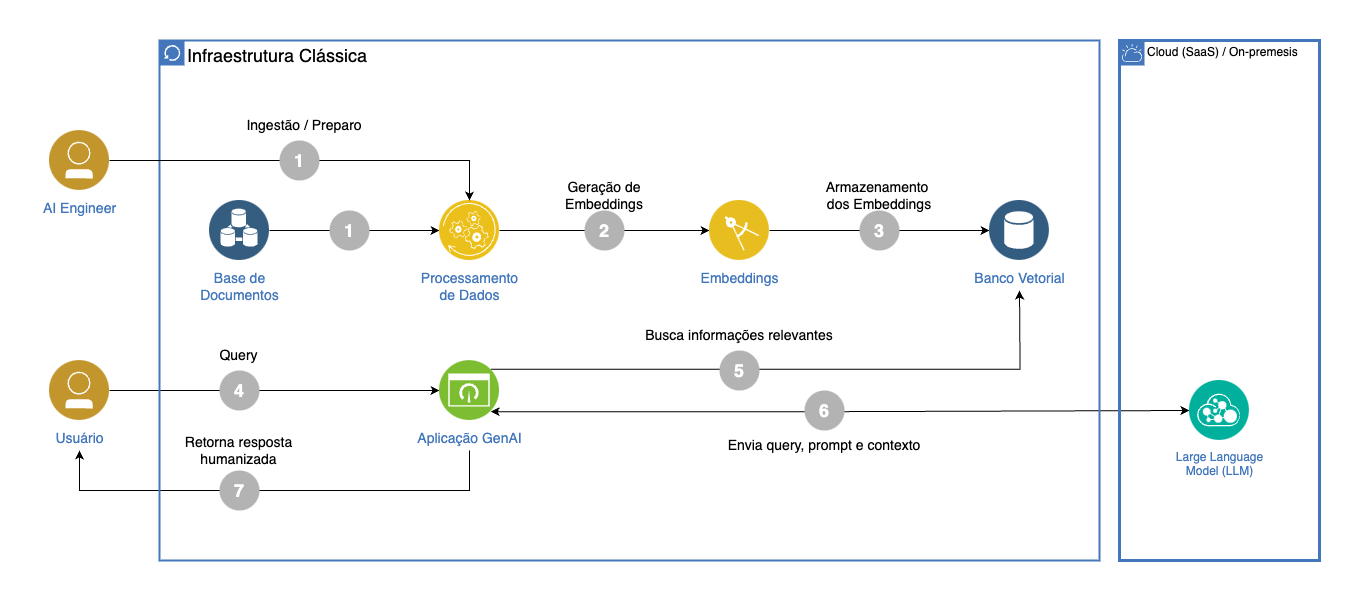
\includegraphics[width=\textwidth,height=0.9\textheight,keepaspectratio]{architecture.png}
        \centering
        \caption{Visão arquitetural da solução RAG proposta para o trabalho}
        \centering
    \end{figure}

    \subsubsection{Ingestão e Preparo}
    
    Etapa onde a biblioteca é analisada, seus documentos são processados e transformados de maneira sequencial para obtermos um determinado modelo com as informações necessárias de cada documento. Esta etapa é dividida em duas partes, uma de ingestão e outra de preparo.

    \begin{itemize}
        \item \textbf{Ingestão:} Nesta parte os documentos são lidos e sua extensão é análisada, determinando a forma como o documento terá seus dados extraídos. Uma vez analisados, o documento é divididoo em chunks, um bloco de texto com os dados do documento.
        \item \textbf{Preparo:} Para cada chunk obtido na ingestão, é instanciado um modelo contendo os dados gerais do documento, assim como os dados do próprio chunk. Este modelo, em específico, visa uma inserção no banco vetorial que será feita na etapa de armazenamento dos embeddings.
    \end{itemize}

    \subsubsection{Geração de Embeddings}
    
    Antes de armazenar os modelos obtidos na etapa anterior, a informação de cada chunk precisa estar em um formato específico para o banco vetorial, este formato é obtido quando geramos os embeddings, que neste contexto, são uma representação numérica de baixa dimensão dos dados de um chunk expecífico.

    \subsubsection{Armazenamento dos Embeddings}
    
    Uma vez gerados, os embeddings de cada chunk estão presentes no modelo previamente adquirido na etapa de Ingestão e Preparo. Nesta etapa ocorre o armazenamento dos modelos na instância do banco vetorial do projeto. O armazenamento é feito de forma sequencial, porém em batches ou grupos com tamanho baseado na quantidade de chunks obtidos. Isso ocorre pois reduz o tempo da etapa de inserção ao banco, tendo em vista que uma vez que um documento é particionado em chunks, dependendo do tamanho do documento, podemos obter mais de 100 chunks, ou seja, 100 inserções.

    \subsubsection{Query}
    
    Aqui ocorre a interação do usuário com o sistema, nesta etapa o usuário digita uma pergunta dentro do espaço de input ou entrada da interface gráfica, que neste contexto é composta por um chat.

    \subsubsection{Busca por informações relevantes}
    
    No momento em que o usuário realiza a query, o sistema realiza uma busca por contexto ou informações relevantes como a biblioteca que o usuário está consultando (caso hajam múltiplas bibliotecas), uma determinada data, autor ou demais filtros que o usuário possa vir a fazer. Com as informações relevantes analisadas, é gerado um objeto de contexto que contém todas as informações relevantes

    \subsubsection{Envio de Query, Prompt e Contexto}
    
    Com o contexto e a query em mãos, o sistema prossegue com o fluxo principal e envia uma solicitação a API contendo a query que o usuário realizou, o prompt a ser seguido pela LLM e o contexto.

    \subsubsection{Retorno de Resposta Humanizada}
    
    Ao final da requisição feita pelo usuário, a API responde com uma lista contendo os objetos presentes no banco vetorial cujo embedding contém informações relevantes para a query do usuário. Esta lista contém os modelos presentes no banco vetorial, definidos na etapa de Preparação, e a partir dessa resposta passamos a lista para uma LLM que irá analisar primeiramente um prompt focado em entregar respostas humanizadas para o usuário. Neste prompt, há todo um cuidado para que qualquer desenvolvedor que deseje implementar este projeto possa utilizar do prompt engineering a fim de realizar as afinações necessárias para seu próprio contexto.

    \subsection{Tecnologias}

    \subsubsection{Python e Ambientes Virtuais}
    
    O Python 3.11 é uma das versões mais recentes da linguagem de programação Python, lançada com melhorias significativas em desempenho, novas funcionalidades e correções de bugs. Uma das principais inovações dessa versão é a otimização do tempo de execução, com um aumento significativo na velocidade em relação às versões anteriores, devido a melhorias no interpretador e na execução de código. Além disso, a versão 3.11 introduziu aprimoramentos na sintaxe, como a simplificação de anotações de tipos e novos recursos que facilitam o desenvolvimento de aplicativos mais robustos e eficientes. A linguagem continua a ser uma das mais populares, especialmente em áreas como desenvolvimento web, ciência de dados e inteligência artificial.
    
    Ambientes virtuais são espaços isolados onde é possível instalar e gerenciar dependências específicas de um projeto, sem afetar o sistema global ou outros projetos. Em Python, esses ambientes são criados com o módulo venv, permitindo que cada projeto tenha suas próprias versões de pacotes e bibliotecas. Isso evita conflitos entre dependências e facilita o gerenciamento de diferentes versões de pacotes para cada projeto.

    As principais vantagens dos ambientes virtuais incluem a capacidade de isolar dependências, garantindo que cada projeto utilize a versão correta de pacotes, a facilidade de replicar e compartilhar ambientes de desenvolvimento e a redução de problemas de compatibilidade entre pacotes ou versões do Python. Eles oferecem um controle mais preciso sobre o ambiente de execução, tornando o desenvolvimento mais seguro e eficiente.

    \subsubsection{Docling}
    Uma biblioteca Python projetada para facilitar a extração e organização de documentos. Ela permite que desenvolvedores processem automaticamente documentos de diferentes formatos, como PDFs, textos e arquivos de Word, para extrair informações estruturadas e relevantes. A biblioteca é útil para automatizar tarefas de leitura e processamento de grandes volumes de dados, organizando-os de forma a facilitar a análise posterior.

    A principal vantagem do Docling é a sua capacidade de simplificar o processo de extração de dados, tornando-o mais rápido e eficiente, sem a necessidade de escrever código complexo para lidar com diferentes tipos de documentos. Isso a torna uma ferramenta valiosa para projetos que requerem análise de texto ou a criação de bancos de dados a partir de documentos não estruturados.

    \subsubsection{Llama Index}
    Uma biblioteca Python que oferece ferramentas para criar índices eficientes, que podem ser usados em conjunto com modelos de linguagem, como o GPT, para realizar tarefas de busca e processamento de texto com alta performance.

    A principal vantagem do LlamaIndex é sua capacidade de organizar dados complexos de forma que seja fácil e rápido realizar consultas sobre eles, integrando-se bem com outras ferramentas de IA e processamento de linguagem natural. Isso a torna útil para criar soluções que necessitam de pesquisa e análise de grandes quantidades de informações, como em assistentes virtuais, sistemas de recomendação e análise de documentos.

    \subsubsection{Elastic Search}
    O ElasticSearch é um serviço de banco de dados baseado em busca de texto completo e análise de grandes volumes de dados. Ele é amplamente utilizado para armazenar, pesquisar e analisar dados de forma rápida e escalável. Baseado no motor de busca Apache Lucene, o ElasticSearch permite que dados sejam indexados e consultados com alta performance, suportando operações como pesquisa por palavras-chave, agregações e análises em tempo real.

    Em um banco vetorial, como o ElasticSearch, os dados são representados como vetores, o que permite consultas de similaridade, ou seja, encontrar documentos que sejam semanticamente semelhantes aos dados consultados. Isso é especialmente útil em casos de busca por texto, recomendação de conteúdo ou sistemas de recuperação de informações avançados. O ElasticSearch organiza e indexa esses vetores para proporcionar consultas eficientes e rápidas, sendo um componente essencial em sistemas que exigem grandes volumes de dados e análises complexas.

    \subsubsection{Ollama}
    A LLM do Ollama é uma ferramenta de inteligência artificial focada em fornecer modelos de linguagem avançados para tarefas como processamento de texto, geração de conteúdo, tradução, resumo e respostas a perguntas. Desenvolvido para ser altamente eficiente e acessível, o Ollama oferece modelos de linguagem que são otimizados para uma variedade de aplicações, desde automação de processos até assistência personalizada em diferentes domínios.

    A principal vantagem da LLM do Ollama é sua facilidade de integração em soluções de software, além de seu desempenho rápido e preciso. A plataforma é projetada para ser simples de usar, com uma interface intuitiva e suporte a diferentes linguagens de programação, tornando a tecnologia de IA mais acessível para desenvolvedores e empresas. Com um foco em flexibilidade e escalabilidade, o Ollama facilita a implementação de modelos de linguagem em larga escala sem comprometer a eficiência.

    \subsubsection{Fast API}
    Um framework moderno e de alto desempenho para construção de APIs em Python. Ele é baseado em padrões como Python type hints e pydantic, permitindo que desenvolvedores escrevam código de forma rápida e eficiente, com uma validação de dados robusta. O FastAPI se destaca pela sua velocidade, sendo capaz de processar requisições de maneira extremamente rápida, o que o torna ideal para aplicações que exigem alta performance.

    As principais vantagens do FastAPI incluem sua facilidade de uso, a validação automática de dados, a documentação interativa gerada com o Swagger UI, e sua performance comparável a frameworks como Node.js e Go. Além disso, o FastAPI aproveita os recursos de tipagem do Python, o que resulta em um código mais claro e com menos erros, além de ser altamente escalável e fácil de integrar com outras ferramentas.

    \subsubsection{Streamlit}
    Uma biblioteca em Python usada para criar interfaces web interativas de forma rápida e simples, sem a necessidade de conhecimentos avançados em desenvolvimento front-end. Ele permite que desenvolvedores criem dashboards, visualizações de dados e aplicativos interativos com poucos comandos, utilizando apenas Python. O Streamlit é ideal para protótipos rápidos e aplicativos que precisam integrar visualizações com análises de dados.

    As principais vantagens do Streamlit incluem sua simplicidade de uso, já que permite criar interfaces com poucas linhas de código, e sua integração direta com bibliotecas como Pandas, Matplotlib e Plotly, facilitando a visualização e análise de dados. Além disso, ele permite a criação de aplicativos interativos com atualizações em tempo real, sem a necessidade de configurar complexos sistemas de front-end. Isso torna o Streamlit uma opção excelente para cientistas de dados e desenvolvedores que desejam criar interfaces intuitivas sem precisar aprender HTML, CSS ou JavaScript.

    \clearpage

    \section{Solução Desenvolvida}

    Com uma visão geral de como funciona um ecossistema RAG e quais artefatos são necessários para implementá-lo, prosseguiremos para o desenvolvimento da solução deste projeto. Levando em consideração as tecnologias apresentadas anteriormente, os próximos tópicos irão abordar o desenvolvimento concreto da solução buscada para este projeto.

    Para a implementação da solução descrita, a biblioteca utilizada foi de todos os trabalhos de conclusão de curso do ano de 2023 publicados pela secretaria do Bacharelado em Sistemas de Informação da Universidade Federal do Estado do Rio de Janeiro, UNIRIO.

    \subsection{Pipeline de Ingestão}
    
    Tendo em vista que uma biblioteca de documentos contém diversos documentos e cada documento possui sua própria extensão, é necessário desenvolver uma solução capaz de processar diversos tipos de documentos, podendo atender diversas bibliotecas distintas.

    Este processamento foi implementado seguindo um Design Pattern, mais especificamente o factory design pattern. O factory design pattern implementa uma interface para a criação de objetos que herdam de uma superclasse, permitindo que as classes filhas possam alterar o tipo de objeto criado. Neste contexto, foi implementada uma fábrica de extratores, todo extrator possui uma instancia dos clientes provedores de serviços do LlamaIndex e Docling, assim como variáveis pré definidas e os métodos de extração.
    
    No entanto, cada extrator implementa o método de extração a sua própria maneira, assim é possível implementar a extração de um arquivo .pdf ou .docx mudando somente a implementação de um único método. Isso contribui para uma melhor manutenção do código e atribui a responsabilidade de extração para um único extrator específico de cada documento.

    Após extraídos os dados dos documentos, é necessário separar os dados relevantes de cada documento e particionar o mesmo em chunks. Para isso, antes de particionar os documentos é realizada uma busca por dados relevantes do documento, neste caso, por se tratar de uma biblioteca de TCCs os dados relevantes são o resumo (abstract), nome, biblioteca a qual ele pertence, caminho (filepath), extensão e mídias do arquivo.

    As mídias são separadas em dois tipos, imagens e tabelas, durante a primeira leitura do documento a biblioteca Docling identifica as mídias dos documentos e as salva em um diretório específico dentro do código do artefato do pipeline, posteriormente este diretório será injetado no código do artefato da API.

    As informações relevantes devem então ser extraídas no começo da extração do documento, uma vez que a busca pelo resumo do trabalho pode tomar tempo de processamento, seria imprudente realizar uma busca após a partição dos documentos. Uma vez extraídas, é gerado um breve resumo do abstract por uma LLM, neste caso foi utilizado o Ollama com um prompt que enfatiza o resumo de no máximo 2 paragrafos contendo 250 caracteres. Essas informações nos geram o seguinte modelo:

    \begin{lstlisting}
        {
            "abstract": "resumo extraído do documento",
            "summary": "um breve resumo do abstract",
            "filename": "nome do arquivo sem extensão",
            "database": "biblioteca a qual o arquivo pertence",
            "filepath": "caminho onde o arquivo se encontra",
            "medias": {
                "images": "lista com o caminho das imagens achadas no arquivo",
                "tables": "lista com o caminhos das tabelas achadas no arquivo"
            },
            "extension": "extensão do arquivo"
        }
    \end{lstlisting}

    Com as informações gerais acima, podemos dar continuidade a partição dos documentos em chunks. Neste projeto, cada chunk possui 2048 tokens. Cada chunk gerado será lido e terá o embedding gerado para a inserção no banco vetorial, neste projeto o modelo de embedding é parametrizado mas optei por seguir esta implementação utilizando o modelo impira/layoutlm-document-qa pois é um modelo especifico para RAG e já treinado para melhor atender nosso caso de uso. Assim, obtemos o seguinte modelo para os chunks:

    \begin{lstlisting}
        {
            "_id": "chave única do chunk",
            "chunk": "objeto imutável obtido durante partição",
            "sequence": "sequência do chunk em questão",
            "pages": "lista de páginas com a informação do chunk em questão",
            "tables": "lista de caminhos das tabelas achadas no arquivo",
            "figures": "lista de caminhos das imagens achadas no arquivo",
            "vector": "embeddings gerado para o chunk"
        }
    \end{lstlisting}

    Este processo de leitura e processamento irá se repetir diversas vezes até que o último documento seja devidamente processado. Uma vez processados, os documentos estarão no formato de chunk seguindo o modelo acima e estarão prontos para inserção no banco vetorial. A inserção no banco irá selecionar cem chunks e realizar uma inserção em batch dos mesmos, devido ao tamanho da biblioteca em questão cem foi um número razoável de chunks, mas dependendo da biblioteca será necessário aumentar este número.

    \subsection{Interface de Programação de Aplicações}
    \lipsum[3-4]

    \subsection{Interface Gráfica de Usuário}
    \lipsum[5-6]

    \clearpage

    \section{Conclusão}
    \subsection{Considerações Finais}
    \lipsum[1-2]
    \subsection{Limitações}
    \lipsum[3-4]
    \subsection{Trabalhos Futuros}
    \lipsum[5-6]

    \clearpage

    \section*{Referências}

    \nocite{*}

    % flush section font left
    \sectionfont{\raggedright}
    \printbibliography
    
\end{document}
